 \documentclass[12pt,a4paper,oneside]{article}
\usepackage{amsfonts, amsmath, amssymb,latexsym,amsthm}
\usepackage[english]{babel}
\usepackage{epsfig}
\usepackage{enumerate}
\usepackage{graphicx} 
\usepackage{float}
\usepackage{subfigure}
\usepackage{cancel}
\usepackage{feynmf}
%\usepackage{subcaption}

\numberwithin{equation}{section}

\parskip=5pt
\parindent=15pt

\usepackage[left=1.7cm,top=2.7cm,right=1.7cm,bottom=2.7cm]{geometry}

\usepackage[utf8]{inputenc}
\usepackage{ dsfont }

\setcounter{page}{0}

\numberwithin{equation}{section}
\newtheorem{question}{Question}
\newtheorem{teorema}{Teorema}
\newtheorem{proposicio}{Proposici\'{o}}
\newtheorem{corollari}{Corol$\cdot$lari}
\newtheorem{lema}{Lema}

\theoremstyle{definition}
\newtheorem{remark}{Remark}
\newtheorem{problema}{Problem}
\newtheorem*{solucio}{Solution}
\newtheorem{exemple}{Exemple}
\newtheorem{exemples}{Exemples}
\newtheorem{observacio}{Observaci\'{o}}
\newtheorem{observacions}{Observacions}
\newcommand{\Q}{\mathds{Q}}
\newcommand{\A}{\alpha}
\newcommand{\C}{\mathds{C}}
\newcommand{\Z}{\mathds{Z}}
\newcommand{\R}{\mathds{R}}
\newcommand{\N}{\mathds{N}}
\newcommand{\F}{\mathds{F}}
\newcommand{\B}{\mathcal{B}}
\newcommand{\Irr}{\mbox{Irr}}
\newcommand{\gr}{\mbox{gr}}
\newcommand{\Gal}{\mbox{Gal}}

\def\qed{\hfill $\square$}

\usepackage{fancyhdr}

\pagestyle{fancy}

\lhead{Jorge Rodr\'{i}guez and Javier Beltr\'an}
\chead{}
\rhead{Planning and Aproximate Reasoning}

\cfoot{\thepage}

\bibstyle{plain}
\date{\today}

\begin{document}

% PORTADA
\begin{center}
	\textbf{ }\\[4cm]
	
	\LARGE Practical Exercise 1: Planner\\[0.5cm]
	\textbf{{\Huge The coffee server}}\\[0.5cm]
	\textbf{{\LARGE Planning and Approximate Reasoning}}\\[1.5cm]
	
	{\Large Universitat Rovira i Virgili}\\[2.3cm]
	{\LARGE \textbf{Master in Artificial Intelligence}}\\[0.5cm]
	{\LARGE $1^{st}$ Semester}\\[2.5cm]
	
	\begin{flushright}
		\textbf{\large{Authors:}\\ \normalsize{Javier Beltr\'an\\Jorge Rodr\'iguez\\}}
	\end{flushright}
	\today
\end{center}
\thispagestyle{empty} 
%\maketitle
\pagebreak

\section{Introduction to the problem}

For this first laboratory we were asked to consider the following scenario:

There is a squared building composed by 36 offices, which are located in a matrix of 6 rows and 6 columns. From each office it is possible to move (horizontally or vertically) to the adjacent offices. The building has some coffee machines in some offices that can make 1, 2 or 3 cups of coffee at one time.
The people working at the offices may ask for coffee and a robot called “Clooney” is in charge of serving the coffees required. Each office may ask for 1, 2 or 3 coffees but not more. The petitions of coffee are done all at early morning (just when work starts) so that the robot can plan the service procedure. Each petition has to be served in a single service.
The goal is to serve all the drinks to all the offices in an efficient way (minimizing the travel inside the building, in order to not disturb the people working).

We start with a initial state called $e_i$, which is compounded of a set of predicates. The initial state in particular has the following predicates: The initial position of the robot, the position of the coffee machines, and position of the coffee petitions.  The final state $e_f$ on the other hand, is compounded of the following predicates: The final robot position and the machines position (no more petition appears). The way of achieving this final state is by going to the machines, take the coffee and them going to each petition to leave the coffee.

To solve this problem we will implement a general planner which later will be use to solve the problem, for this we will use an algorithm called STRIPS. This algorithm is based on stacking the predicates needed to get to the final state and them finding the operators needed to get this predicates. The implementation of this has been done in Java, this will be explained in detail bellow.

As we mentioned before to formalise this problem we need to define a set of predicates and operators, for each operator we have series of preconditions, adds and deletes which are sets of predicates. This is shown in the Table\ref{op} all this together with the arguments needed for each operator:

\begin{table}[h!]
	\centering
	\caption{ Table with operators and its adds, deletes and preconditions}
	\label{op}
	\begin{tabular}{|c|l|l|l|}
		\hline
		Opertors    & \multicolumn{1}{c|}{Preconditions}                                                          & \multicolumn{1}{c|}{Adds}                                                             & \multicolumn{1}{c|}{Deletes}                                          \\ \hline
		Make(o,n)   & \begin{tabular}[c]{@{}l@{}}robot-location(o)\\ robot-free\\ machine(o,n)\end{tabular}       & robot-loaded(n)                                                                       & robot-free                                                            \\ \hline
		Move(o1,o2) & \begin{tabular}[c]{@{}l@{}}robot-location(o1)\\ steps(x)\end{tabular}                       & \begin{tabular}[c]{@{}l@{}}robot-location(o2)\\ steps(x+distance(o1,o2))\end{tabular} & \begin{tabular}[c]{@{}l@{}}robot-location(o1)\\ steps(x)\end{tabular} \\ \hline
		Serve(o,n)  & \begin{tabular}[c]{@{}l@{}}robot-location(o)\\ robot-loaded(n)\\ petition(o,n)\end{tabular} & \begin{tabular}[c]{@{}l@{}}served(o)\\ robot-free\end{tabular}                        & \begin{tabular}[c]{@{}l@{}}petition(o,n)\\ robot-loaded\end{tabular}  \\ \hline
	\end{tabular}
\end{table}
%%%%%%% Table with the operators, precondtions, adds ad deletes

The predicates are easier to define, the following list show the predicates considered for this problem:

\begin{itemize}
	\item \textbf{Robot-location(o)}: the robot is in office o.
	
	\item \textbf{Robot-free}: the robot has no cup of coffee.
	
	\item \textbf{Robot-loaded(n)}: the robot has n cups of coffee.
	
	\item \textbf{Petition(o,n)}: office o wants n cups of coffee.
	
	\item \textbf{Served(o)}: office o has been served, no more coffee is needed in this office.
		
	\item \textbf{Machine(o,n)}: there is a coffee machine in office o that produces n cups of coffee each time (with n equal to 1, 2 or 3).
	
	\item \textbf{Steps(x)}: the total distance travelled by the robot (calculated with Manhattan distance).
		
\end{itemize}

There are some consideration that can be taken so the problem is simpler:

\begin{itemize}
	\item The robot only makes coffee for a single petition each time. That is, the robot cannot make 3 cups of coffee to serve two different offices. First, will make coffee of one office and serve it, and after will go to the same or another coffee machine to serve the second office.
	
	\item If a petition is of n cups, the robot will make coffee only with a unique machine of capacity n. That is, the robot cannot make coffee with 2 or more machines and accumulate the cups to serve a unique petition.
	
\end{itemize}


\section{Analysis of the problem}

In this section we are going to  analyse the problem. First of all we notice that to the given initial state we have to  add robot-free, as to the goal state.

Taking into account the considerations to simplify the problem, this problem can be seen as an optimization problem where we want to minimize the number of steps of the robot choosing the order in which it has to visit every petition after passing for a coffee machine with the same amount of coffee as the petition. 

The search space has a total size of $|P!||M^{|P|}|$, where $|P|$ is the number of petitions and $|M|$ the number of possible machine, supposing that the robot always takes the optimal path form one point to another, so the number of possible paths is irrelevant,as the cost is always the same. To get to this result we just need to notice that we have two list of possible orders, the petitions which can't be revisited, what means a factorial; and the machines which can be revisited what means a exponential number of combinations. As we can see the number of petitions is what increases more the complexity of the problem, interestingly the complexity rely on the number of petitions and machines, the size of the grid doesnt' affect the complexity.

For the example we have a total of 375000 possible solutions, however as we have taken the consideration that to serve a petition we need to go to a machine with the same number of coffees, the total number decreases to 1920.

Solving the problem with an standard exploration algorithm is not an option, we must use a different one, for this exercise we will use the STRIPS algorithm. STRIPS has a linear cost, however is does not find the optimal solution, unless we use the correct heuristics. This heuristics we have defined are explained in the next section.

Another thing to take into account is that, in the definition of the problem the robot moves across a square grid consisting of 36 squares, the squares are called o1, o2, ..., o36. To make it easier to count the number of steps, we have considered a way to convert this to coordinates $(x,y)$. For a $6 \times 6$ grid we have the following equation:

\begin{align}
	x & = o-1 \ (mod6) \\
	y & = [\frac{o-1}{6}] 
\end{align}

Where o is the value of the position, $[ \ ]$ represents the integer part of the number and  $mod6$ means the remainder of the division.

Since this is an example, the preconditions, operators and states are quite straightforward, however the way the steps are calculated could somehow be troublesome. This doesn't mean is difficult, we just need to be careful as we do it in the implementation.

For the STRIPS algorithm we need to organize well the preconditions as new operators are needed, if we do not do so, we can situations like cycles or impossible to instantiate parameters. For example, if we use the operator $Make(o,n)$ if the precondition $robot-location(o)$ the one in the top of the stack, the algorithm would not know the value of $o$, instead, if we stack $Machine(o,n)$ last, the value $o$ is given by the number of coffees $n$ needed. In the following section we will discuss the heuristics needed to avoid this kind of situations and to minimise the steps needed to serve the coffees.


\section{Planning algorithm}

The first think we have to consider is the order we stack the predicates for the final state, as this is the way we  will resolve the problem, the order determines directly the optimality. To solve this we have created two functions:
\begin{itemize}
	\item The first one orders the petitions based on the distance to the final position. This way we solve the problem trying to end the nearest as possible from the final position. This does not assure optimality but it gives a decent enough solution.
	
	\item The second one, orders the petitions based on their distance to the first and last locations. The way it does this is by staking first the nearer to the final location, them it stack last the nearest to the initial location, etc. This approach is slightly better than the previous one, since we take into account the initial location. Nevertheless, as before, we can't assure the optimality of the solutions, sometimes it will be optimal. Although, we know that the solution will very suboptimal.
	
\end{itemize}

For the operators $Make$ and $Serve$ we have chosen a fix order to stack the preconditions, since the order determines the result of the problem. For this we have done some steps of the STRIPS algorithm by hand, so we could see how the algorithm works for our problem.

For the $Make$ operator, first we stack $robot-location$, since we do not know the value for the $o$ parameter; them we stack $Machine$ so we can get the location $o$ based on the petition value $n$, notice that the location of the machine will be the nearer one to the robot and the petition, in other words, the one that minimises, $d$:
$$d = distance(machine, robot) + distance(machine, petition)$$
 At last, $robot- free$ gets stacked, since is the first think need before getting coffee, notice that the way we have define this problem, the robot will always be free when it gets here.
 
 For $Serve$ operator the order is more or less the same. First we stack $robot-location$, since we do not know the value of $o$; them $robot-loaded$, due to it has to carry coffee to serve it and we do not know the number of coffees needed; the last thing to stack, which will be the first thing to get unstacked, is the petition which will instantiate the values of $o$ and $n$.
 
 Summarizing the planner will stack $Served(o)$ then it will unstack it, to get to $Served(o)$ we need the operator $Serve(o,n)$ which has the preconditions: $robot-location(o)$, $ loaded(n) $ and $petition(o,n)$. with petition it instantiates the parameters, the planner unstacks loaded, for which it needs the operator $Make(o',n)$ after stacking the preconditions: $robot-location(o')$, $machine(o',n)$ and $robot-free$. It instantiates $o'$ so it can use the operator $Move(o_i,o')$. Them the planner has solved one petition, the rest are exactly the same.

\section{Implementation design}

\subsection{A generic approach of the linear planner}
Given that the problem consists in building a planner for a concrete solution (the coffee server), we believe that the best approach is to design a generic planner, which can be used for modelling any linear planning problem by just extending it.

For achieving this, and taking into account that the program is built in Java, we followed an Object-Oriented approach. That is, every element of the algorithm has to be part of the model of the program. So the first task is to identify the main components of the STRIPS algorithm with a stack of goals:

\begin{itemize}
	\item The \textbf{stack} itself, which is a data structure with a LIFO policy. It contains all kinds of elements that are part of the problem, like the predicates and the operators.
	\item The elements to be stacked, specifically:
	\begin{itemize}
		\item The \textbf{predicates}. They define the state of the problem and have 0 or more parameters, which can be instantiated or not.
		\item The \textbf{operators}. They define how a state changes, by removing some predicates and adding others. They also have parameters which can be instantiated or not.
		\item A \textbf{set of predicates}. They have to be added at some steps to make sure that we did not lose any predicate in order to achieve another one. There is a special case: the final \textbf{state} of the problem, which also has to be added to the stack as a set of predicates.
	\end{itemize}
	\item As we have seen before, \textbf{parameters} are needed. They are just a key-value item, but the value may have been instantiated or not. When a parameter gets a value, all the appearances of the parameter in the stack must be updated with the new value. For example, a parameter in our problem might be "o", and it may take values from "o1" to "o36".
\end{itemize}

It can be seen that many different kinds of objects have to be stored in the same stack. Also, we need access to all the elements pushed to the stack, not only the one on the top, so we can instantiate all the appearances of a parameter. Our proposal is the following: we can use the $Stack<E>$ from \textit{Java Collections}. It solves our two main concerns because of these reasons:

\begin{itemize}
	\item It grants access to each element stored with $get(int i)$, so we can instantiate all appearances of a parameter.
	\item It is a generic stack, so it can be used to store objects of any type. But this type has to be the same. We solved this by constructing a \textit{marker interface} called $Stackable$. This means that every object that can be stacked must inherit from the $Stackable$ Java interface.
\end{itemize}

Our architecture for the Stackable elements is the following:

(image of stackable elements)

The linear planning algorithm is executed in the \textbf{LinearPlanner} class. It needs some information about the problem to solve: the initial and final states, the available operators and the available predicates. It is also responsible for logging the execution of the algorithm so it is easier to debug. One can see that the Linear Planner is a complex object that requires multiple attributes and some constraints among them. For example, the predicates that compose the initial and final state should be consistent with the available predicates defined.

In order to make the task of creating a Linear Planner easier for the user, we added a \textit{LinearPlannerBuilder}. It is a \textit{Builder} pattern that helps in creating such a complex object. It also informs the user about errors or inconsistences in the declaration of the problem.


\subsection{A specific application: The Coffee Server}

If the problem to be solved is complex enough, just taking the generic planner and declaring the specific predicates, operators and states may not be enough. For example, some operators may have a special behaviour, that cannot be imitated by the generic Operator.

This is what happens in our Coffee Server. The $Move(o1,o2)$ operator, when applied, deletes the $Steps(x)$ predicates and adds $Steps(x + distance(o1,o2))$, where $distance(o1,o2)$ is the Manhattan distance between cells $o1$ and $o2$. We cannot use the generic Operator we built, because it just replaces some predicates for others, keeping the same parameters.

These problems can be solved by extending the generic Planner module, and adding some specific elements with a special behaviour. In our case, a MoveOperator has been created. It is able to instantiate the parameter of $Steps$ properly, by increasing the path distance and saving it in the new predicate.

The heuristics used by the solver are also problem-specific, and should extend from the $Intelligence$ interface. In our problem we define the heuristics explained in the previous section. They implement the methods $orderFinalState()$ for stacking the petitions in the most efficient order, and $orderPreconditions()$ for stacking the preconditions of every operator and preventing loops.

(full class diagram)

Having explained the common and the specific part, the best way to organize the functionality of this program is to hold a STRIPS package, which contains the generic linear planner; and a coffeeServer package, with the specific part of this problem.

(package diagram)

\section{Testing cases and results}
Thanks to the \textit{ProblemReader}, any CoffeeServer problem can be written and read from the program. One just needs to write the initial and final state, following the syntax indicated in the exercise. Specifically, we have created 5 new problems (and the example one). Their main goal is to test the efficiency of the method, in terms of optimality of the solution and execution time.

\subsection{Optimality of the problem}
The STRIPS linear planner does not achieve an optimal solution, but we can try to improve its results by using good heuristics. We explained our heuristics in previous sections, and here we present how they work. We will do this by comparing the results obtained for the example problem.

\begin{figure}[!h]
	\centering
	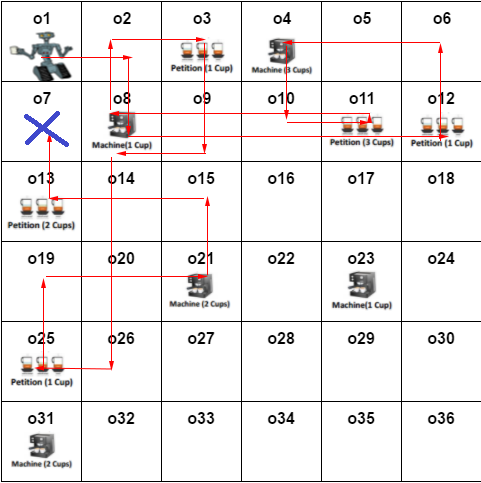
\includegraphics[scale=0.7]{figures/example_problem.png}
	\caption{Example problem and the sub-optimal path found}
	\label{example_optimality} 
\end{figure}

The steps taken by the algorithm are 29. We know that this is sub-optimal, as it is higher than the number of steps indicated in the exercise definition.

Our conclusion is that our heuristics may be improved by taking into account not only the final position of the robot, but also the starting position, so as to organize the petition orders in a logical way for minimizing displacements.

\subsection{Performance metrics}
The number of steps taken to solve the problem is not the only measure we should try to minimize. Given that the algorithm iterates over the stack in order to apply operators and build a plan, there are multiple ways to get to a plan in a specific number of steps. And some of these plans are more efficient than others (they require a least amount of iterations of the algorithm). This is why we are also looking at the number of iterations to complete the problem. The number of iterations is proportional to the execution time, which is another measure we are trying to optimize. 

Now we are presenting the 5 problems created for testing the planner. They have an increasing number of petitions, which is the predicate directly related to the complexity of the solution. The following image shows the initial state of every problem, as well a blue cross in the final position they must achieve. Please note that the definition of these problems in text files is found in the project, as well as their logs. For formatting reasons, you may find them in the Annex 1 of this document.

The performance results for these problems are presented in the following table, in the measures of number of steps, iterations and execution time in milliseconds.

\begin{table}[]
	\centering
	\caption{My caption}
	\label{my-label}
	\begin{tabular}{llllll}
		\hline
		Problem             & \textbf{P1 (4)} & \textbf{P2 (6)} & \textbf{P3 (10)} & \textbf{P4 (20)} & \textbf{P5 (31)} \\ \hline
		\textbf{Steps}      & 42          & 65          & 42          & 149         & 180         \\
		\textbf{Iterations} & 82          & 120         & 196         & 386         & 595         \\
		\textbf{Time (ms)}  & 101         & 113         & 159         & 332         & 647         \\ \hline
	\end{tabular}
\end{table}

The number of steps depends on the disposition of the petitions themselves, so it is not a good measure for general performance of the algorithm. We will focus on the iterations and the execution time. The following graphics show their evolution.

\begin{figure}[H]
	\centering
	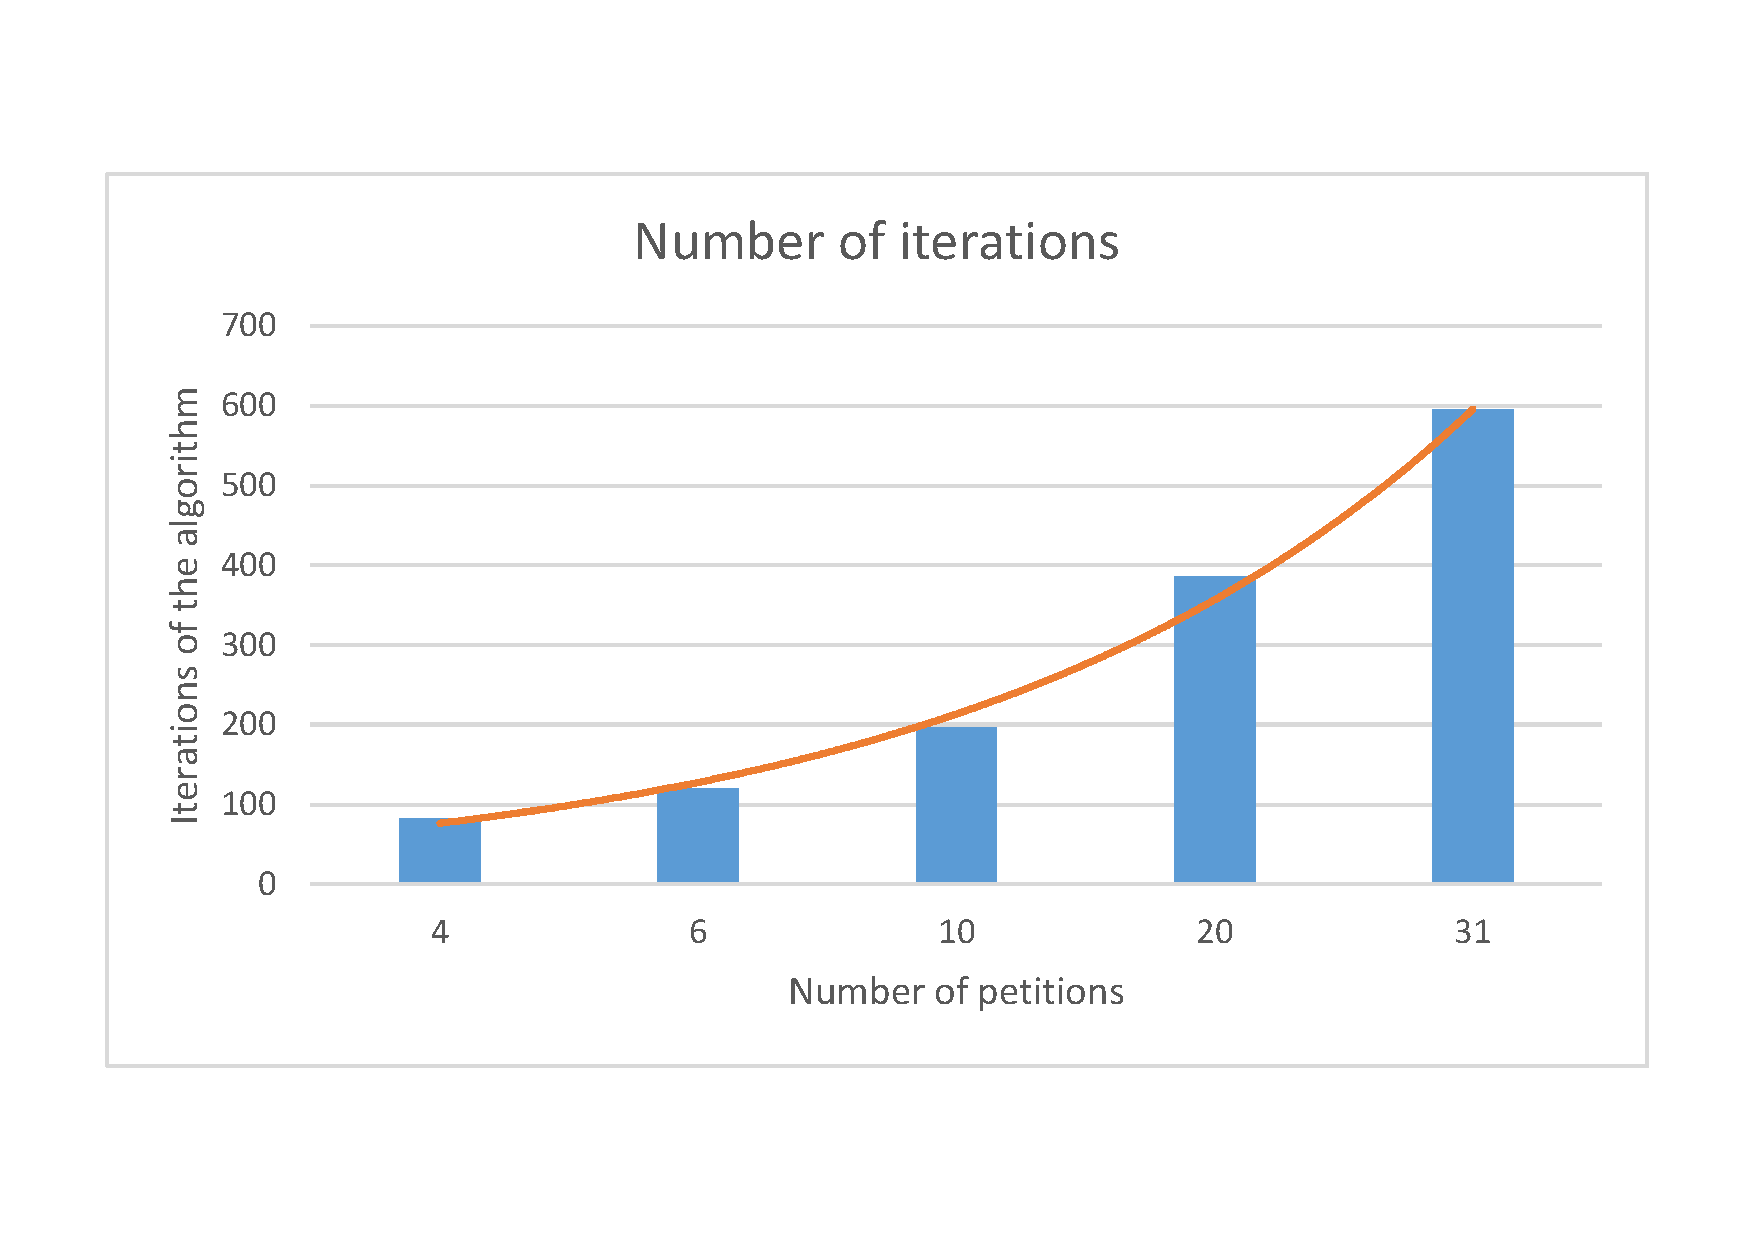
\includegraphics[scale=0.4]{figures/iterations.pdf}
	\caption{Evolution of the iterations as the petitions increase}
	\label{iterations} 
\end{figure}


\begin{figure}[H]
	\centering
	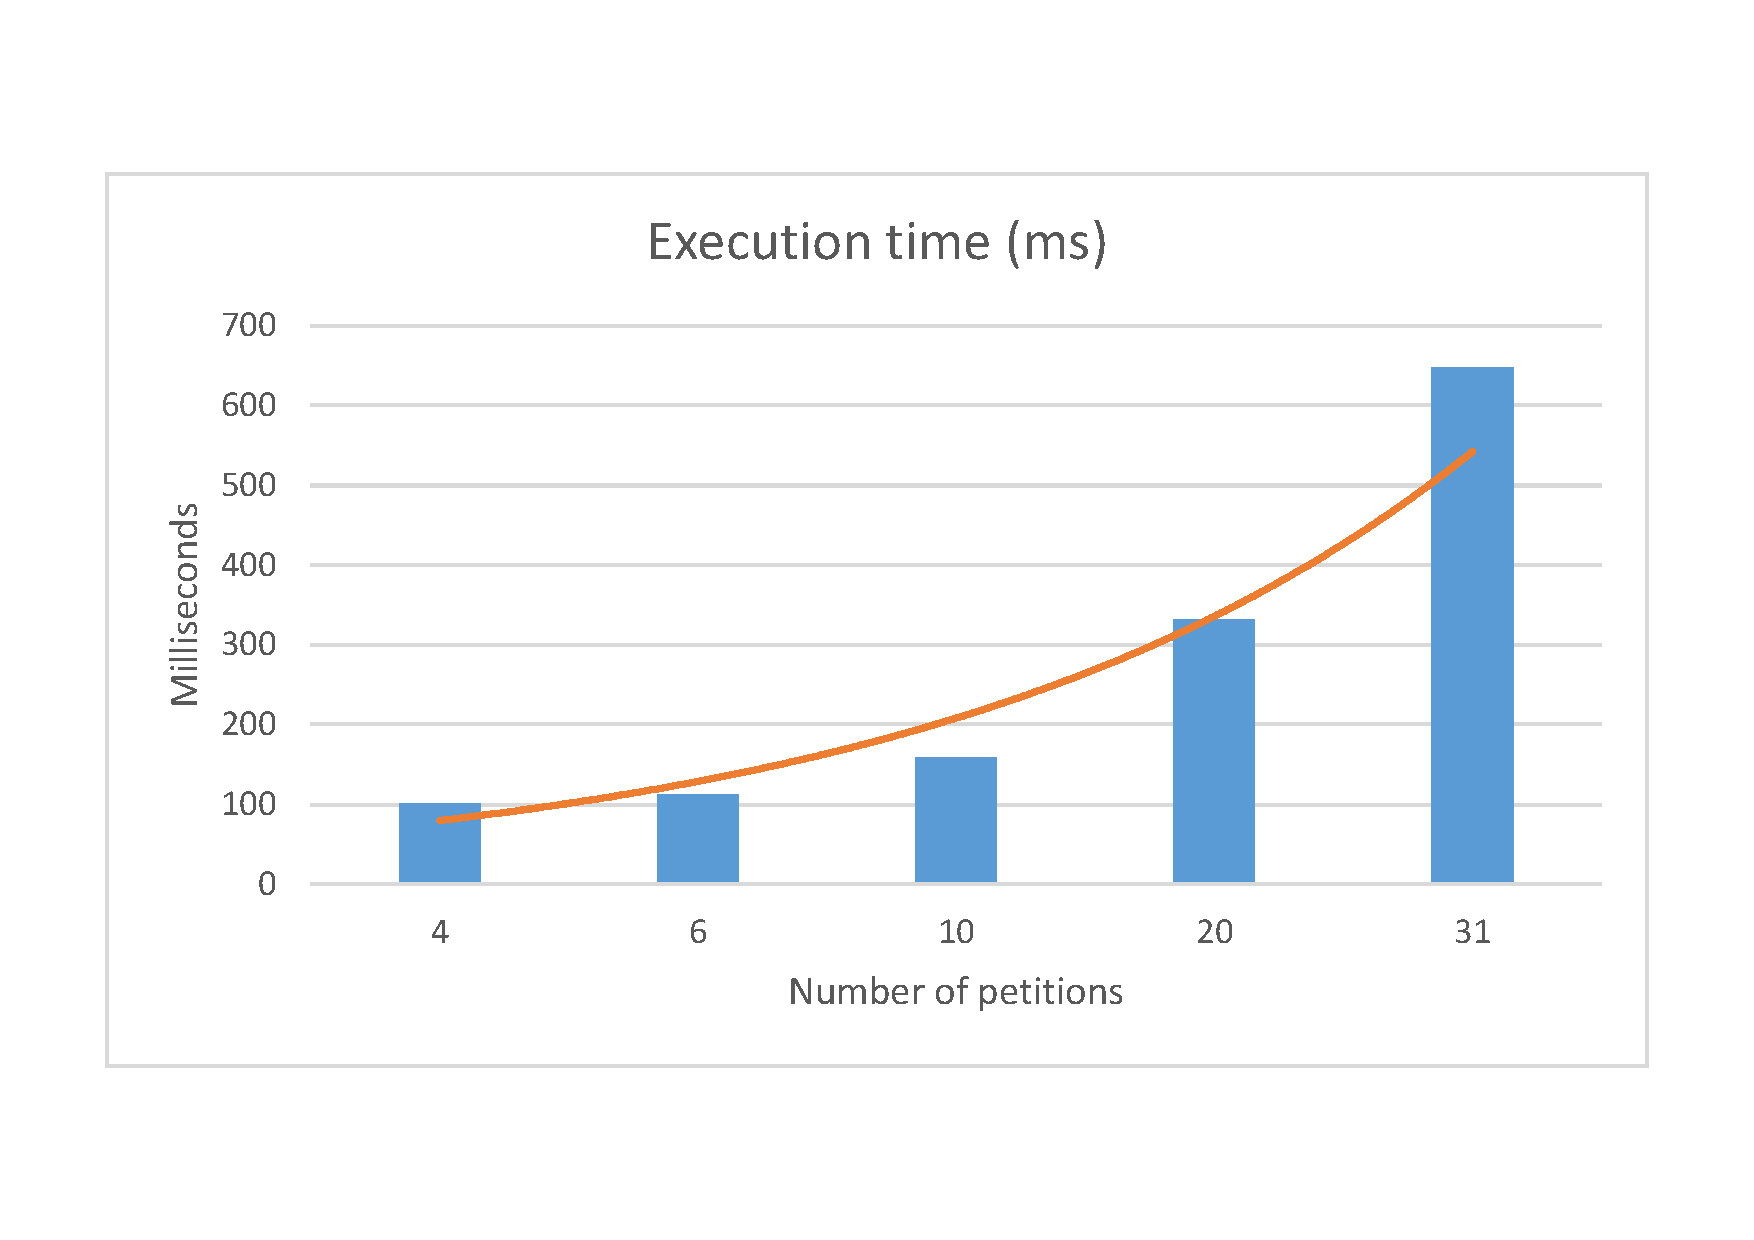
\includegraphics[scale=0.4]{figures/time.pdf}
	\caption{Evolution of the time as the petitions increase}
	\label{time} 
\end{figure}

In both cases (which are profoundly related) the values follow an exponential trendline. This leads us to think that this method becomes impracticable for problems bigger than the ones for the coffee server, which are limited by the grid size.

\section{Instructions to execute the program}

\newpage
\section{Annex 1: definition of the test problems}
\begin{figure}[!h]
	\centering
	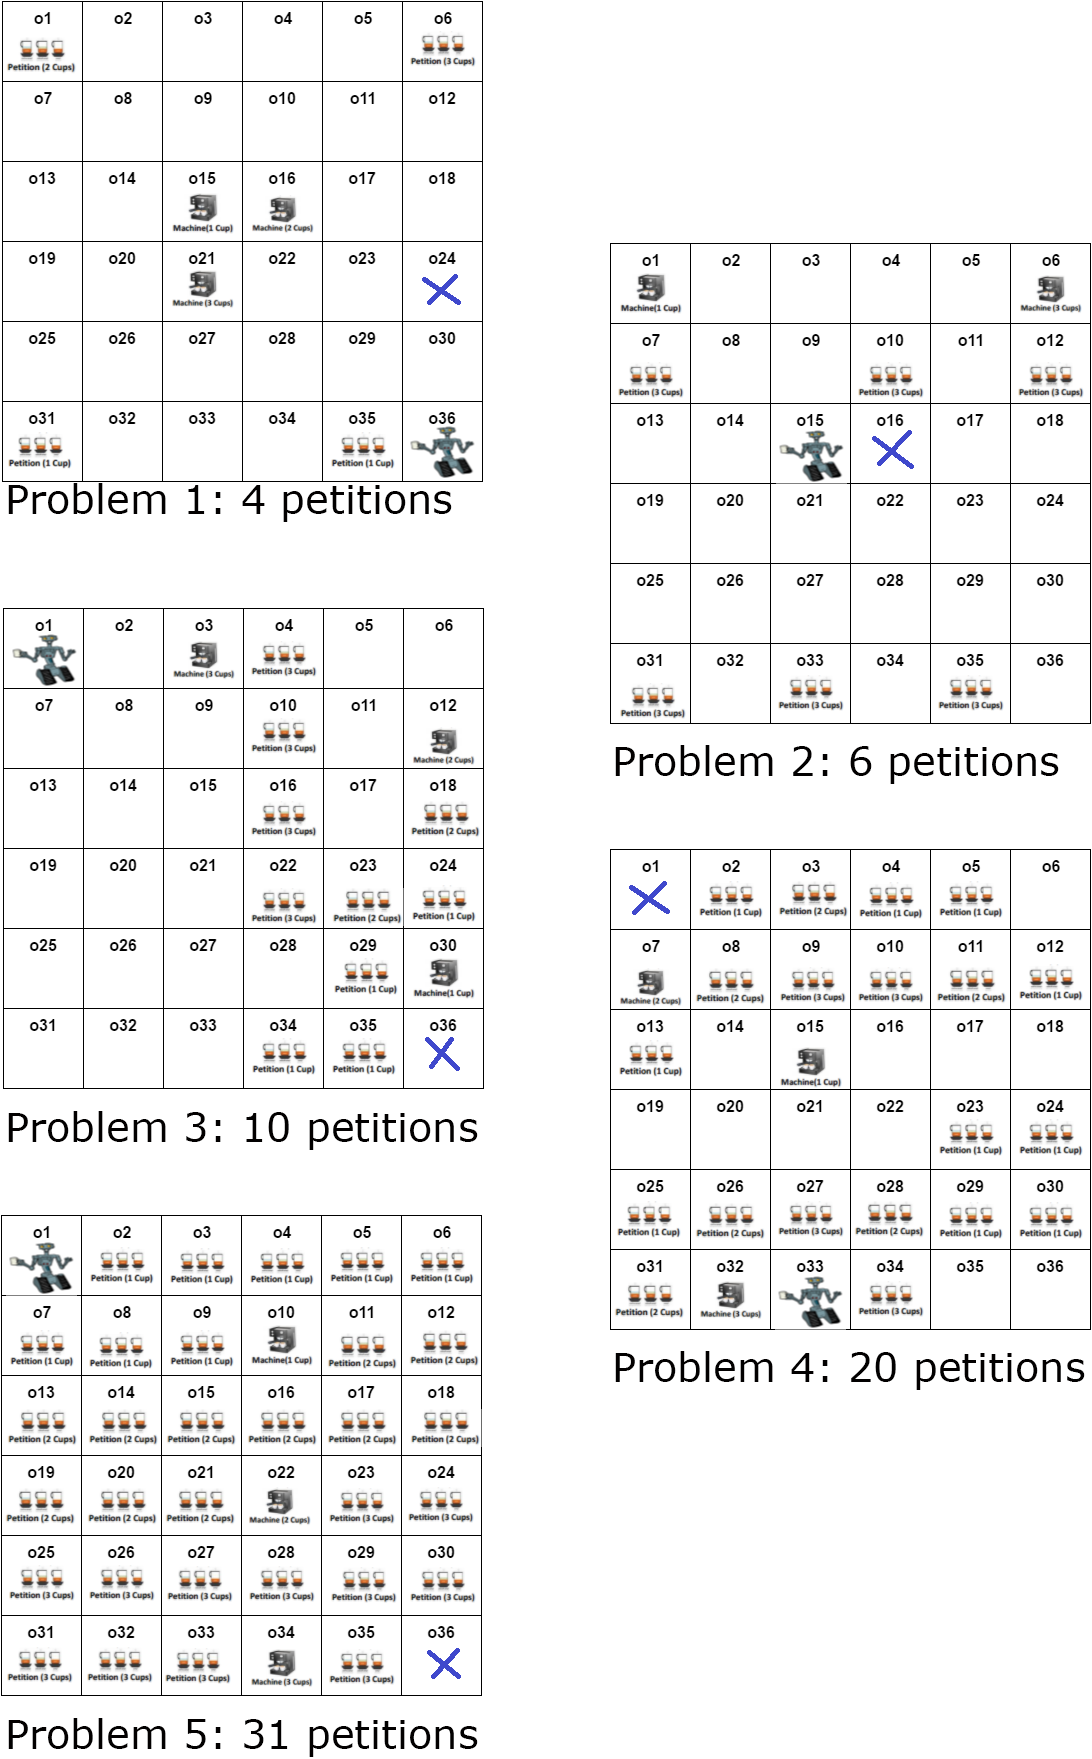
\includegraphics[scale=0.4]{figures/problems.png}
	\caption{Definition of the 5 test problems}
	\label{problems} 
\end{figure}

\end{document}
